\section{sosa}
\label{sec:sosa}
%%%%%%%%%%%%%%%%%%%%%%%%%%%%%%%%%%%%%%%%%%%%%%%%%%%%%%%%
\begin{figure}[h!]
\begin{center}
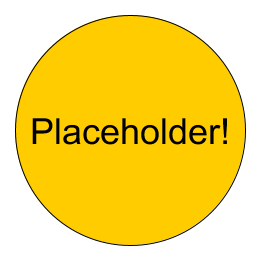
\includegraphics[width=.8\textwidth]{figures/placeholder}
\end{center}
\caption{Schema Diagram for the sosa Pattern. The visual notation is explained in Chapter \ref{chap:prelims}.}
\label{fig:sosa}
\end{figure}
\subsection{Summary}
\label{sum:sosa}
%%%%%%%%%%%%%%%%%%%%%%%%%%%%
I am some summary text.

%%%%%%%%%%%%%%%%%%%%%%%%%%%%%%%%%%%%%%%%%%%%%%%%%%%%%%%%
\subsection{Axiomatization}
\label{axs:sosa}
%%%%%%%%%%%%%%%%%%%%%%%%%%%%
\begin{align}
% General Axioms\top &\sqsubseteq \forall\textsf{place.Holder} \\ 
\exists\textsf{place.Holder} &\sqsubseteq \top 
% Domain and Range Restrictions\top &\sqsubseteq \forall\textsf{place.Holder} \\ 
\exists\textsf{place.Holder} &\sqsubseteq \top 
% Inverse Aliases (if any)placeholder &\equiv holderplace^- 
\end{align}

%%%%%%%%%%%%%%%%%%%%%%%%%%%%%%%%%%%%%%%%%%%%%%%%%%%%%%%%
\subsection{Explanations}
\label{exp:sosa}
%%%%%%%%%%%%%%%%%%%%%%%%%%%%
\begin{enumerate}
\item temporary item
\end{enumerate}

%%%%%%%%%%%%%%%%%%%%%%%%%%%%%%%%%%%%%%%%%%%%%%%%%%%%%%%%
\subsection{Competency Questions}
\label{cqs:sosa}
%%%%%%%%%%%%%%%%%%%%%%%%%%%%
\begin{enumerate}[CQ1.]
\item temporary item
\end{enumerate}

\newpage
%%%%%%%%%%%%%%%%%%%%%%%%%%%%%%%%%%%%%%%%%%%%%%%%%%%%%%%%
% End Section
%%%%%%%%%%%%%%%%%%%%%%%%%%%%%%%%%%%%%%%%%%%%%%%%%%%%%%%%
%%%%%%%%%%%%%%%%%%%%%%%%%%%%%%%%%%%%%%%%%%%%%%%%%%%%%%%%